\section{Framework Composition}\label{sec:physical_analysis} 
The physical layer defines the electrical and physical framework for receiving and 
transmitting signals through the media, and furthermore it defines encoding/decoding 
and alignment schemes for translating frames into signals and visa versa.

This project requires the use of DTMF tones as information carrier, and furthermore it is
required that transmission are broadcast through the air. These requirements decides some
of the properties of the physical layer, the first one is the media which is the air as 
sound waves are used for communication, and the communication can only take place as half-duplex as sending and receiving is impossible as the communication system works as a broadcast system.

\nomenclature{DTMF}{Dual-tone multi-frequency}

	\subsection{DTMF as information Carrier}
	DTMF is an abbreviation for Dual Tone Multiple Frequency. It is a system of tones that are used by
	telephones when dialing a number. The system is an arrangement of four low tones and four high tones,
	they are arranged in a four-by-four matrix which gives the system sixteen combinations.
	
	The idea is that these sixteen combinations formed by the DTMF matrix is used to transmit data
	between two or more computers. To let DTMF tones enter into data communication we have
	to apply the property of  waves to carry bits. This can be done by letting each entry in the matrix
	consist of four bits. Four bits gives sixteen combinations which each can be assigned to an entry in
	the matrix. Below is shown the DTMF map which will be used in the physical layer for encoding and decoding.
	
	\begin{table}[!h]
		\begin{center}
			\begin{tabular}{c|c c c c}
			 & 1209 Hz & 1336 Hz & 1477 Hz & 1633 Hz \\
			\hline
			697 Hz & 0000 & 0001 & 0010 & 0011 \\
			770 Hz & 0100 & 0101 & 0110 & 0111 \\
			852 Hz & 1000 & 1001 & 1010 & 1011 \\
			941 Hz & 1100 & 1101 & 1110 & 1111 \\
			\end{tabular}
		\end{center}
		\caption{Table of the matrix with the bit combinations assigned to each entry.}
		\label{tab:DTMF_mapping}
	\end{table}
	
	Now by letting one computer play the tones through a speaker and another computer record it from
	a microphone then data is transmitted. The exchange of data is essentially an exchange
	of information and it is not satisfying exchanging information of the size of four bits alone,
	cause this would make the system inefficient. The system need to be able to transmit a sequence
	of tones matching a given bit pattern. The number of tones played each second will determine the
	bit rate of the communication. As each tone hold four bits the bit rate can be written as below:
	\begin{equation}bitrate = \frac{numberOfTones \cdot numberOfBitsPerTone}{time}\end{equation}
	
	\subsection{Utilisation of PortAudio Interface}
	PortAudio exposes streams for recording or playing back sound through the sound card of a
	computer. PortAudio allow for developers to push raw audio data to the soundcards outgoing buffer and
	receiving raw audio data from the soundcards ingoing buffer. Thus, PortAudio is good foundation for the
	implementation of the physical layer as tone detecting, and tone generating algorithms can be laid on top
	of PortAudio, as basic mathematics which apply to digital signal processing. The PortAudio API provides the
	user with a callback function which implicitly exposes the sound card buffers for input and output. PortAudio
	furthermore gives the possibility for using more sound streams which then provide more callback functions
	which means that input and output streams can run asynchronously. The way PortAudio handles these streams
	will be explained in greater detail later.
	
	PortAudio will be implemented as a part of the physical layer to create the interface between the developed
	protocol stack and the sound card. Figure \ref{fig:physical_4layers} show the components which forms the physical layer. 
	
	\begin{figure}[!h]
		\begin{center}
		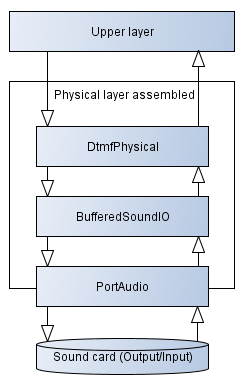
\includegraphics[scale=0.6,trim=0 0 0 0]{content/graphics/physical/physical_4layers.png}%trim=l b r t
		\caption{Assembly of components in the physical layer. DtmfPhysical handles frames and BufferedSoundIO handles DTMF tones.}
		\label{fig:physical_4layers}
		\end{center}
	\end{figure}
	
	The DtmfPhysical and BufferedSoundIO will be implemented as two separated classes which will be bounded together
	and exposed as the physical layer to the rest of the protocol stack. The idea for implementing the physical layer
	as two seperate classes on top of PortAudio API, is to separate functionality between the physical layers internal
	layers. BufferedSoundIO class will be implementing the math needed to generate and detect tones while the physical
	layer class will implement the encoding schemes for transforming frames from the data link layer into a sequence of
	numbers which then can be pushed to BufferedSoundIO which then processes this sequence to generate a sequence of DTMF
	tones at the sending site. In the receiving site the receiving process will look a lot like the process for sending a
	frame, the BufferedSoundIO class will detect sequences of DTMF tones which will be transformed into a sequence of
	numbers. This sequence of numbers will then be sent to the DtmfPhysical and then be translated into a frame.
	
	\subsection{Goertzel Algorithm}
	To be able to detect if tones have been transmitted some algorithm for detection of tones have to be implemented.
	For this purpose the Goertzel algorithm is used, this algorithm has the ability to detect if a signal contain a
	specific frequency. Other algorithms exist which would provide the same information but those would be
	much more expensive regarding the computational complexity. Those other algorithms are called Discrete Fourier Transform (DFT)
	
	\nomenclature{DFT}{Discrete Fourier Transform}
	\nomenclature{FFT}{Fast Fourier Transform}
	
	and the other is called Fast Fourier Transform (FFT) which is a more efficient way to obtain the same information
	as the DFT algorithm. The number of operations of DFT \cite[p. 124]{DSP} is $N^2$, where N is the number of samples.
	For FFT \cite[p. 124]{DSP} the number of operations is calculated to be $\frac{N}{2}\cdot log_{2}(N)$,
	where N is the number of samples.
	
	As the detection of tones has to occur as fast as possible it is desired to lower the cost of cpu power by using 
	an algorithm which has the least computational complexity. The Goertzel algorithm therefore suit this need very well.
	The reason for this is that with a few pre-calculated constants and N iterations over N samples, a value is returned
	which indicate if a specific frequency is present in the incoming signal.
	
	Essentially the Goertzel algorithm is a second order IIR filter which is dependent on current input and previous
	output, the filter is given as the difference equation \ref{eq:physical_goertzel_sequence}.
	\begin{equation}y(n) = x(n) + 2\cdot cos(2\pi \cdot f_{0})\cdot y(n - 1) - y(n - 2),\end{equation}\label{eq:physical_goertzel_sequence}
	where $f_{0}$ is the frequency of interest.
	
	By Z-transform the following is obtained:
	\begin{equation}H(z) = \frac{Y(z)}{X(z)} = \frac{1}{1 - 2\cdot \cos(2\pi \cdot f_{0})\cdot z^{-1} + z^{-2}}\end{equation}
	
	\nomenclature{IIR}{Infinite Impulse Response}
	
	As the above equation show, it is a second order IIR filter. This can be implemented as a direct form-II structure, as illustrated on figure \ref{fig:physical_biquad_filter} where the point W is of interest.
	
	\begin{figure}[!h]
		\begin{center}
		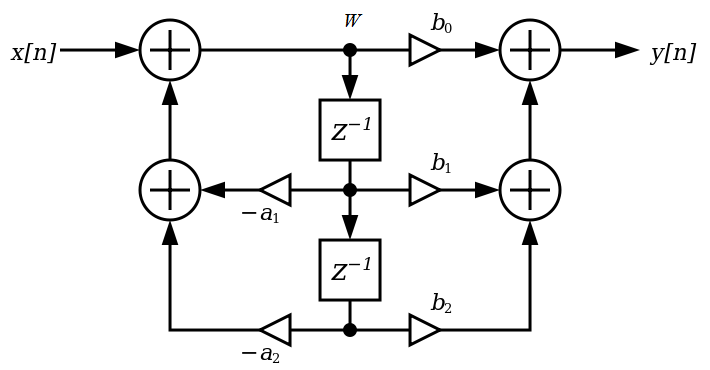
\includegraphics[scale=0.6,trim=0 0 0 0]{content/graphics/physical/physical_biquad_filter.png}%trim=l b r t
		\caption{A direct form II implementation}
		\label{fig:physical_biquad_filter}
		\end{center}
	\end{figure}
	
	The point W will be used for calculating the frequency response at a specific frequency of interest. As this is taking
	place in discrete time, an expression of the frequency of interest is needed. In discrete time the frequency spectrum
	is divided into frequency bins, the size of these bins is determined by the number of samples and the sample rate.
	Obtaining the k'th bin can be done as shown below:
	\begin{equation}k = \frac{f_{0}}{f_{s}}\cdot N\end{equation}
	where $f_{0}$ is the frequency of interest, $f_{s}$ is the sampling frequency, and N is the number of samples.
	
	Now it is possible to calculate the filter coefficients, which in the case with the Goertzel algorithm reduces 
	to one single coefficient. This coefficient have to be calculated for each tone that want to be identified, but can 
	be calculated in advance because its only dependent on the frequency of interest.
	
	The coefficient is calculated with:
	\begin{equation}c = 2\cdot cos(2\pi \cdot \frac{k}{f_{s}})\end{equation}
	
	Now that all constants can be calculated in advance the detection system only have to calculate the filter output, calculate
	the magnitude of the frequency and then it is able to decide based on the result if the frequency exist in a incoming signal.
	As detection of DTMF tones is needed for this application it needs to determine if two specific frequencies is present at the
	same time. But this wont be much of a problem as the constants for each frequency can be calculated in advance.
	The algorithm are implemented as a direct form-II structure, and need to iterate over the array of collected samples to be
	able to detect if a given frequency is present in a signal.
	
	The computational complexity can therefore be written as one multiplication plus two additions per iteration per tone.
	This leads to:
	\begin{equation}numberOfOperations = 3\cdot N\cdot M,\end{equation}
	where N is the number of samples and M is the number of tones.
	
	For one tone detection over 205 samples this is around 600 calculations, for detection of 8 tones simultaneously the equation
	above result in around 5000 calculations, and these are real calculations where as for DFT and FFT the computational complexity 
	is much higher and the calculations are carried out with complex numbers.
	
	This is the reason for choosing the Goertzel algorithm for detection of frequencies.
	
	\subsection{Synchronisation}\label{sec:physical_sync}
	The physical layer will be handling the synchronisation of the data stream. Keeping the data in sync enables the software to
	keep track of the given chunks of data from the upper layer, this is important to do because the physical layer at the receiving
	site will have to assemble the DTMF tones back into the exact same chunks of data for delivery to the upper layer.
	A way to solve this need is to wrap the content of data into a header and possibly a tail. The chuck of data received from the 
	data link layer would be natural to wrap in a header and a tail as an extra precaution to indicate if the frame is transmitted.
	This will ease the assembly of a frame because the software have an indication of the exact start of a frame and the exact ending
	of it as well.
	
	Another problem with synchronization arise due to the mapping between 4 bit combinations and DTMF tones. This is because if there is a
	need for sending, 1111 and 1111 right after each other the system will not be able to identify the two tones corresponding to the
	given bit patterns from each other. It would therefore look like only one tone was transmitted instead of two. This actually apply
	to each combination which are followed up by its own combination of bits. Some kind of stuffing is needed to separate each tone
	from each other.
	
	There are several ways in which this problem can be solved. One of the possibilities is to stuff the transmitted tones with a little
	bit of silence in between each other. This implementation would require some sort of timing scheme which would rely on precise timing
	so decisions, on how the recorded silence should be interpreted, can be made. Decisions that will define the transmission of a frame, will be as 
	already mentioned, where does a frame start, where does it end, and the stuffing in between each tone. All these properties will be
	hard to manage due to silence can be considered as white noise which is totally random. White noise is not in the scope of this 
	document.
	
	A second solution could be to do the stuffing at the data link layer in between equal bit patterns with a another bit pattern. 
	The are several disadvantages duo to use of this method. First the synchronization would now be spread across two layers because
	the physical layer still would have to track the beginning of a frame and the end of a frame. Another disadvantage is that this 
	method is unreliable as the defined bit pattern for stuffing at the data link layer could be generated by the data contained by the 
	frame itself. This mean that when data containing the bit pattern for stuffing this data could be discarded on false reasons and
	then corrupt the frame.
	
	A third and more elegant solution is to add a ninth frequency to the map seen in table \ref{tab:DTMF_mapping}.
	
	\begin{table}[!h]
		\begin{center}
			\begin{tabular}{c c|c c c c}
	 		index & & 0 & 1 & 2 & 3 \\
			& DTMF & 1209 Hz & 1336 Hz & 1477 Hz & 1633 Hz \\
			\hline
			0 & 697 Hz & 0 & 1 & 2 & 3 \\
			1 & 770 Hz & 4 & 5 & 6 & 7 \\
			2 & 852 Hz & 8 & 9 & 10 & 11 \\
			3 & 941 Hz & 12 & 13 & 14 & 15 \\
			4 & 350 Hz & 16 & 17 & 18 & 19 \\
			\end{tabular}
		\end{center}
		\caption{This new mapping system create four new combinations of DTMF tones. The index notation can be used for
		implementation purpose.}
		\label{tab:newDTMF_mapping}
	\end{table}
	
	In table \ref{tab:newDTMF_mapping} a new mapping of DTMF tones is shown. This new mapping system contain four new combinations of tones
	which can be used as control signals. The combination $1209 Hz$ and $350 Hz$ gives the number 16, this number could be used as a code for
	\textit{here does the frame start}, 17 for \textit{here does the frame end}, and 18 for \textit{two equal bit patterns are presented after
	each other}. Code 19 can be leaved as a reserved control code. 
	
	\begin{table}[!h]
		\begin{center}
			\begin{tabular}{|c|c|}
			\hline
			\textbf{Code} & \textbf{Representation}\\
			\hline
			16 & Start of a frame \\
			\hline
			17 & End of a frame \\
			\hline
			18 & Double tone \\
			\hline
			19 & \textit{Reserved} \\
			\hline
			\end{tabular}
		\end{center}
		\caption{Show a table of control codes(tones).}
		\label{tab:physical_control_tones}
	\end{table}
	
	This method for synchronization is also well connected to the rest of the
	data transmission at the physical layer as the implementation is based on a tone detection system, so by adding an extra tone a lot of new
	possibilities are offered, in exchange of complicated timing schemes or sharing the synchronization functionality between two layers.
	The detection system can now by identifying a shift in tone frequencies detect a new tone was sent and thus the system is able to
	register the tone.
	
	\subsection{Encoding scheme}\label{sub:encoding_scheme}
	The encoding and decoding will be handled on two levels, the encoding from frames to a sequence of 4 bit data elements and control codes, and the decoding of sequences to frames is handled in the DtmfPhysical class. The encoding from a sequence code to DTMF tone and decoding in opposite direction is handled in the BufferedSoundIO class.
		
	The encoding and decoding happening in the DtmfPhysical class is based on the synchronisation method that was chosen in section \ref{sec:physical_sync}. The encoding of a frame into a code sequence is pretty straight forward, as the system will extract the three bytes which a frame consist of, as six nibbles. The system will analyse these nibbles to see if any of them have an identical nibble next to it, if so the sequence of nibbles is stuffed with 18 which corresponds to \textit{Double tone} according to table \ref{tab:physical_control_tones}. After this stuffing has taken place the frame is wrapped in a \textit{begin} and \textit{end} signature. An example of this is shown below:
	
	\begin{table}[!h]
		\begin{center}
			\begin{tabular}{|c|c|c|c|c|c|}
			\hline
			12 & 1 & 1 & 15 & 10 & 11 \\
			\hline
			\end{tabular}
		\end{center}
		\caption{Representation of a random frame as the six nibbles.}
		\label{tab:physical_frame}
	\end{table}
	
	The process explained before would result in the code sequence represented in table \ref{tab:physical_control_tones}:
	
	\begin{table}[!h]
		\begin{center}
			\begin{tabular}{|c|c|c|c|c|c|c|c|c|}
			\hline
			16 & 12 & 1 & 18 & 1 & 15 & 10 & 11 & 17 \\
			\hline
			\end{tabular}
		\end{center}
		\caption{Represent a frame as the code sequence after stuffing it.}
		\label{tab:physical_stuffed_frame}
	\end{table}
	
	The decoding of a code sequence into a frame works a little different as the physical layer is able to run asynchronously and the internal data stream are independent of each other. This causes that incoming data wont look like the data that was sent. Lets say that the PortAudio callback is fired twice as often on the receiving computer as the sending computers output callback and otherwise out of synchronisation, this lead to a received code sequence which could look like the one in table \ref{tab:physical_received_frame}.
	
	\begin{table}[!h]
		\begin{center}
			\begin{tabular}{|c|c|c|c|c|c|c|c|c|c|c|c|c|c|c|}
			\hline
			16 & 12 & 12 & 1 & 1 & 18 & 18 & 1 & 1 & 15 & 10 & 11 & 11 & 17 & 17 \\
			\hline
			\end{tabular}
		\end{center}
		\caption{Represent a random received code sequence which represent a frame.}
		\label{tab:physical_received_frame}
	\end{table}
	
	Decoding of this sequence requires for the system to identify control code from actual data codes. This i done by ignoring the numbers 16, and 17, as a sequence will always be arranged in frames because a sequence always start with 16 and ends with 17. The next thing is that the system needs to iterate over the sequence to remove all the codes the match up with the previous code. When it meets 18 the decoding scheme know that two identical codes are allowed next to each other in the frame. This process will result in the frame mentioned in table \ref{tab:physical_frame}.
	
	The encoding and decoding which is taking place in the BufferedSoundIO class can be considered as a table look up for now. For further insight of the mathematics going on behind the scenes it is recommended to look at appendix \ref{app:physical_encode}.